\chapter{Brain structural connectivity}

The transfer of information and functional integration between different parts of the brain is influenced by white matter connections. The relationship between brain structure and function is still under active research, and the degree to which function is dependent on the structure is not entirely clear. However, there is no doubt that the relationship exists. \cite{sotiropoulos_building_2019} In this work, we focus on the prediction of brain function, specifically its reaction to a stimulus, using the structure. 

Mapping billions of individual neurons in the human brain is intractable. Because of that, we attempt to use a simplified description of the structure while keeping its important properties. Structural connectome describes the structure of white matter fiber pathways as a graph. Vertices represent parts of the brain, and edges represent their anatomical connections. The connectome is usually represented as a connectivity (adjacency) matrix. \cite{yeh_mapping_2021}

The first section of this chapter describes the process of obtaining structural connectome. The following section is devoted to the specific connectomes used in this work.

\section{Structural connectome acquisition}

\TODO[v \cite{yeh_mapping_2021} je hezký obrázek 2, možná překreslit a použít?]

Structural connectome construction aims to give a macroscopic view of the brain structure. The problem consists of two parts. First, we have to define how to divide continuous grey matter into areas forming nodes. Second, we have to estimate the length and \enquote{strength} of the white matter fiber bundles connecting these nodes to add weighted edges to the graph.

There are various approaches how to obtain structural connectome, both invasive and non-invasive. In this work, we consider diffusion-weighted magnetic resonance imaging (DW-MRI) and tractography, which is a non-invasive approach. It is an indirect method (it does not explicitly measure the quantity of interest) and because of that, it suffers from several limitations, extensively described in a paper The Seven Deadly Sins of Measuring Brain Structural Connectivity Using Diffusion MRI Streamlines Fibre-Tracking by Calamante et al. \cite{calamante_seven_2019}. Because of that, it is error-prone, and the results should be treated with caution. \cite{sotiropoulos_building_2019}

\subsection{Node definition using brain parcellation}

As described in Section \ref{sec:MRI}, the result of the MRI is a 3D image. The next step is dividing continuous grey matter, represented by voxels in the 3D image, into a bearable number of discrete nodes. The resulting division is called parcellation, and the parcels/nodes are called regions of interest (ROI). 

The simplest and most common approach how to obtain brain parcellation is using one of so-called anatomical atlases. An anatomical parcellation atlas is a standardized map of the brain based on anatomical features such as neural macrostructures (for example, sulci and gyri -- depressions or furrows and ridges on the cerebral cortex). Atlas-based image recognition works as follows: For a sample patient image, objects in the image can be recognized by registration of the sample image with the atlas image. By aligning corresponding points between the sample and atlas images, the labels assigned to regions in the atlas image can be transferred and applied to the sample image. \cite{sotiropoulos_building_2019, lawrence_standardizing_2021,chang_ljchangdartbrains_2020,rohrer_focused_2008} 

There are various parcellation atlases stemming from various anatomical or functional perspectives. Created through a range of techniques, these parcellations enable various insights into the brain organization and network properties. However, the use of different parcellations across studies brings difficulties when comparing different studies and complicates reproducibility. The parcellations vary not only in the number of nodes but also in their positions. Because of that, results may vary; while one parcellation may reveal a particular effect, it might not be observable with another parcellation. \TODO[odkázat na část, kde budu psát o svých pokusech] \cite{sotiropoulos_building_2019, lawrence_standardizing_2021}

Lawrence et al. made an effort to standardize the human brain parcellations in the Neuroparc project available on GitHub\footnote{\url{https://github.com/neurodata/neuroparc}}. For a nice summarization of various approaches to brain parcellation and a list of parcellation atlases, let us also recommend \textit{Introduction to Parcellations}\footnote{\url{https://dartbrains.org/content/Parcellations.html}, accessed 1. 5. 2024} by Sava-Segal and Botch (part of an online coursebook DartBrains by Luke Chang). \cite{chang_ljchangdartbrains_2020}

\subsubsection{Node coordinates}

It is useful for the subsequent network analysis to keep the information about the spatial distances of the nodes. Because of that, we need to assign 3D coordinates to each node. The coordinates are obtained as a center of mass of the voxels registered as a part of the region of interest. They could be calculated for the atlas \enquote{model brain} or separately for each patient sample. For simplicity, we consider only the first option because we are working with average data, and the small differences are not of interest to us.

\subsubsection{Selected parcellations}

In this work, we came across several parcellations. This section provides their list, including short descriptions. 

\begin{itemize}

    \item \textbf{Yeo}\label{parc:Yeo} \cite{thomas_yeo_organization_2011}: The parcellation is based on the main functional areas in the brain and it was created using data from 1000 healthy subjects using a clustering approach. It divides the brain into 7 or 17 functional areas based on the version.
    
    \item \textbf{Desikan–Killiany (DK)}\label{parc:DK}  \cite{desikan_automated_2006}: The DK parcellation is defined by gyri. It was generated using 40 subjects (30 healthy, 10 with Alzheimer’s disease). It consists of 68 regions, 34 per hemisphere. There is also an updated Desikan-Killiany-Tourville (DKT) \cite{klein_101_2012} version of this parcellation, which merges regions that were not clearly defined. Because of that, DKT has only 62 regions. There is often 
    
    \item \textbf{Schaefer200}\label{parc:Schaefer200}  \cite{schaefer_local-global_2018}: The parcellation is based on functional data from task-based fMRI and resting-state fMRI. There are several versions based on the level of detail, the number of parcels could range from 100 up to 1000. We used a version with 200 parcels. Each parcel also comes with Yeo's 7 Networks label.
    There is a parcellation is available on GitHub.\footnote{\url{https://github.com/ThomasYeoLab/CBIG/tree/master/stable_projects/brain_parcellation/Schaefer2018_LocalGlobal}}
    
    \item \textbf{Glasser}\label{parc:Glasser}  \cite{glasser_multi-modal_2016}: The parcellation is defined using a multimodal approach, combining brain anatomy (myelin content and cortical thickness), function (MRI measured during different tasks), connectivity (resting-state functional MRI) and topography. It is constructed based on data from 210 healthy subjects. It consists of 360 regions, 180 per hemisphere, therefore it is the most detailed parcellation used in this work. It is sometimes denoted as MNI-HCP-MMP1.
    
\end{itemize}

In practice, we encountered several issues with parcellations usage. First of all, when we want to use a publicly available structural connectivity matrix, it is necessary to know not only which parcellation was used but also how the regions of interest are ordered in the matrix. Some authors use alphabetical ordering, while others use ordering based on the spatial proximity of the regions or their functional similarity. The main problem is that the paper does not always indicate the version. Therefore, we recommend being careful when using connectivity matrices from external resources.

Another problem was caused by the fact that the brain parcellation could use various coordinate systems.\footnote{Further information about coordinate spaces can be found in \textit{Coordinate Systems Appendix} of \textit{The Brain Imaging Data Structure} specification. The appendix is available on GitHub \url{https://github.com/bids-standard/bids-specification/blob/master/src/appendices/coordinate-systems.md} (accessed 1. 5. 2024). \cite{gorgolewski_brain_2016}} Because of that, it might be complicated to match data from two different resources even if they have the same parcellation.

\TODO[ještě něco?]

\subsection{Edges estimation}

Conceptually, we want to create a map of long-range white matter fibers connecting the gray matter regions of interest discussed above. 

As explained in Section \ref{sec:MRI}, DW-MRI measures water molecules' diffusion in brain tissues. It gives us information about the intravoxel axon arrangement. Based on this information (combined with some anatomical restrictions), a technique called tractography reconstructs the most probable streamline paths in white matter by tracing the water diffusion direction from voxel to voxel. \cite{yeh_mapping_2021,iturria-medina_characterizing_2007} 

The next step is defining a measure of connectivity between nodes. There are many options, such as the number, length, volume, or probability of streamlines between the corresponding nodes, but the mean value of a diffusion metric itself could also be used. \cite{yeh_mapping_2021} In this work, we use measures based on streamline counts and lengths because these were published by the authors of the connectivity matrices used here.

% https://commons.wikimedia.org/wiki/File:MRI_DWI_sequence_showing_restricted_diffusion_in_the_mesial_dorsal_thalami.jpg
% https://en.m.wikipedia.org/wiki/File:White_Matter_Connections_Obtained_with_MRI_Tractography.png

\section{Group-average structural connectome construction}\label{sec:group-avg}

Assume we already have a connectivity matrix for each subject in some group, edge weights representing streamline count. Because we want to work with the general structural properties of the brain, the question of constructing a group-representative connectome arises. The goal of group averaging is to increase the signal-to-noise ratio and obtain a clearer picture of brain network organization in general while preserving network properties that are consistently expressed at the subject level (such as edge length distribution). \cite{betzel_distance-dependent_2019} In this section, we present some possible approaches.

\subsection{Simple average}\label{sec:average}

The most straightforward idea is to average the streamline count between each pair of nodes across all the subjects. The main problem with this approach is that whenever there is at least one subject with an edge from A to B, the AB average is always non-zero, so it suggests that \enquote{there is a connection between these nodes}. As a result, the network density might be higher in the averaged connectome. That is an issue, especially because the process of obtaining streamline counts is erroneous, and the presence of one subject with this edge might be an accident.

\subsection{Consensus thresholding}\label{sec:cons-thr}

Consensus thresholding is the most common approach. It tries to preserve features consistently expressed at individual subjects' level while reducing noise. Threshold $\tau$ between 0 and 1 is specified\footnote{There is no consensus about the \enquote{correct} value of $\tau$ and it is often selected according to some heuristics. That might be a source of complications while attempting to compare connectomes across different studies.}, and the connections that are observed in at least $\tau$ fraction of subjects are kept. These connections are associated with weight, for example, the average number of streamlines among the subjects where the connection is present. The rest is set to 0. \cite{betzel_distance-dependent_2019}

Betzel et al. point out that this approach favors shorter edges which are easier to reconstruct using tractograpy. Consequently, the distribution of edge lengths is different in average connectome than in the single subjects. According to their argumentation, the longer edges are less common, but despite of that, they have an important function in the brain. On the grounds of that, it is important to keep the edge length distribution because structural networks need long-distance connections. They propose their own method to prevent the issue, and we present it below. \cite{betzel_distance-dependent_2019} 

\subsection{Distance-dependent consensus thresholding}\label{sec:dist-dep}

This method aims to preserve edge length distribution. Assume the list of edges and their lengths.\footnote{Lengths might be Euclidean distances of the nodes or some sort of streamline average lengths.} Let us define $M$ as the total number of edges we want to keep in the consensus network. We define $M$ bins based on edge length percentiles. For each of them, we find all possible edges falling into that bin by length. For each bin, we choose the edge that is expressed most often across the subjects with ties broken by the greatest average weight (for example, streamline count). \cite{betzel_distance-dependent_2019} 

We used \texttt{struct\_consensus} method from netneurotools package\footnote{\url{https://netneurotools.readthedocs.io/en/latest/index.html}} for Python for calculation of distance dependent thresholding during the work on this thesis.

\subsection{Averaging by Rosen and Halgren}\label{sec:rh}

We include the description of this specific method because it was used in one of the matrices we used in our experiments (see Section \TODO). We decided to follow the averaging methodology described by Rosen and Halgren in the paper \textit{A Whole-Cortex Probabilistic Diffusion Tractography Connectome} \cite{rosen_whole-cortex_2021} to get a matrix comparable with the one published by Rosen and Halgren with a different group of subjects.

The principle is the same as a simple average, but it works with ratio of streamlines between two parcels to global number of streamlines instead of plain streamline counts. According to the paper, the values are first averaged across the subjects and than scaled such as the number of streamlines originating at parcel A and terminating at parcel B is divided by the total number of streamlines that either originate at parcel A or terminate at parcel B, excluding within-parcel connections. \cite{rosen_whole-cortex_2021} We used the equation below, where $SC$ is the final structural connectivity matrix and $m$ is an average of structural matrices across individual subjects.

$$
SC_{ij} = \frac{m_{ij}}{\sum_k m_{ik} + \sum_l m_{lj} - (m_{ii} - m_{jj})}
$$

The resulting matrix was sometimes non-symmetric even if the individual subject matrices were symmetric. It was caused by numerical instability in Python while working with small numbers. To overcame this problem, we added $SC = (SC + SC^T) /2$ to the end of the procedure.

\section{Structural connectomes description}

All structural connectomes used in the thesis are described in this section. Some of them were published as group-averaged, while others came as a set of single-subject matrices. This section aims to present how they were constructed and compare their network properties.

\subsection{Enigma}

The first source of structural connectivity matrices for this thesis is a Python package ENIGMA TOOLBOX\footnote{\url{https://enigma-toolbox.readthedocs.io/en/latest/}, accessed 1. 5. 2024} developed by S. Larivière and B. Bernhardt from MICA Lab - Montreal Neurological Institute \cite{lariviere_enigma_2020}. It provides an option to load structural connectivity matrices in several parcellations. The original data were taken from 207 healthy adults from the HCP dataset.\footnote{The Human Connectome Project (HCP) is a large scientific effort focused on mapping the connectivity of the human brain. The HCP datasets are openly available to researchers at \url{https://www.humanconnectome.org/}. \cite{van_essen_human_2012}} The preprocessing pipeline is described in detail in a paper \textit{The ENIGMA Toolbox: Cross-disorder integration and multiscale neural contextualization of multisite neuroimaging datasets} by Larivière et al. For our application, it is important to note that the group average structural connectome was obtained using a distance-dependent thresholding procedure described above \ref{sec:dist-dep}. Afterward, it was log-transformed. The structural connectomes are available in DK, Glasser, and Schaefer parcellations. 

There is a disadvantage of Enigma structural matrices, they provide only edge weights, not lengths. 

\subsection{Domhof}

This dataset, created by Domhof et al. \cite{domhof_parcellation-based_2022}, is available online on EBRAINS platform.\footnote{\url{https://doi.org/10.25493/NVS8-XS5}} The repository provides individual connectomes for 200 subjects from the Human Connectome Project (HCP). For each subject, there is a matrix with streamline counts and a matrix with streamline lengths. They provide the connectomes in 20 different parcellations, including DK and Schaefer200 parcellation. 

During the data investigation, we found that there are 70 ROIs in the matrices in DK parcellation. We removed the surplus ROIs to achieve compatibility with Enigma.

We constructed the group-representative matrices using three approaches described in Section \ref{sec:group-avg}, namely simple average, distance dependent consensus thresholding and Rosen and Halgren method. For streamline lengths group average, we calculated an average considering only the values for which the corresponding weight was non-zero.

\subsection{Mica-Mics}

This dataset was published by Royer et al. \cite{royer_open_2021} on The Canadian Open Neuroscience Platform.\footnote{\url{https://n2t.net/ark:/70798/d72xnk2wd397j190qv}} It consists of multimodal data from 50 healthy adult subjects and there are Glasser and Schaefer200 parcellations available. We constructed the group-representative matrices for both of them using the same approaches as for the Domhof dataset.

\subsection{RosenHalgren}

This dataset was published by Rosen and Halgren. \cite{rosen_whole-cortex_2021} It is again based on data from HCP, this time 1065 healthy adults. The group representative weights and lengths matrices are available on Zenodo\footnote{\url{https://doi.org/10.5281/zenodo.10150880}} in Glasser parcellation. The group-average was created following the averaging procedure described above. 

\subsection{PyTepFit}

The last structural connectivity weights and lengths matrices were taken from a Github repository\footnote{\url{https://github.com/GriffithsLab/PyTepFit/tree/66b94e488c82478e6f302015b6cd8e8d9d33792a/data}} of PyTepFit project by Momi et al\cite{momi_tms-evoked_2023}. These are already group-averaged (simple average) matrices with Schaefer200 parcellation created using data from 400 healthy subjects from the HCP project. 

\section{Structural connectomes comparison}

The goal of this work is to investigate the relationship between structural connectivity and the function of the brain. Before we move to that in Chapter \ref{ch:ftract} and Chapter \ref{ch:pytepfit}, we should explore the structural connectivity itself. It is necessary to understand the nature of structural connectivity and how it differs depending on the data source and preprocessing method before we use it for the prediction of the function.

\subsection{Preprocessing methods}

An important question is, what is the influence of different preprocessing methods on the resulting average connectome? In this section, we chose the Schaefer200 parcellation for the presentation of the results because we have the most data availible in this parcellation. \TODO[The results for the other parcellations are similar and could be seen TODO]

Let us look at simple statistics about the connectivity matrices in Table \ref{tab:sc_stats}. First of all, Rosen and Halgren's method yields overall much lower values, because it uses the ratio of streamlines instead of streamline count. For the other methods, which all use streamline counts as edge weights, consensus thresholding has both the highest mean and median values, while  We also see that the distance-dependent consensus thresholding results in fewer edges than the other methods, which are all the same. 


\begin{table}
\begin{subtable}{\textwidth}
    \centering
    \begin{tabular}{l | c | c | c }
        preprocessing & edges count & mean	& median\\
        \midrule
        simple             &40\,000  &239.4  &15.6	\\
        cons ($\tau=0.75$) &40\,000	&240.0	&16.2	\\
        dist               &33\,750	&239.1	&15.5	\\
        rh                 &40\,000	&0.002	&0.0002 \\
    \end{tabular}
    \caption{Domhof dataset}
    \label{tab:sc_stats}
\end{subtable}

\bigskip

\begin{subtable}{\textwidth}
    \centering
    \begin{tabular}{l | c | c | c }
        preprocessing & edges count & mean	& median\\
        \midrule
        simple             &40\,000  &232.2	&38.6	\\
        cons ($\tau=0.75$) &40\,000	&232.7	&38.9	\\
        dist               &38\,336	&231.6	&37.8	\\
        rh                 &40\,000	&0.001	&0.0001 \\
    \end{tabular}
    \caption{Mica-Mics dataset}
    \label{tab:sc_stats}
\end{subtable}
    \caption[Statistics for structural connectivity group average matrices]{Statistics for structural connectivity group average matrices, Schaefer200 parcellation. Preprocessing methods are: simple -- simple average \ref{sec:average}, cons -- consensus thresholding with $\tau=0.75$ \ref{sec:cons-thr}, dist -- distance-dependent consensus thresholding \ref{sec:dist-dep}, rh -- Rosen and Halgren's method \ref{sec:rh}. }
\end{table}

\begin{figure}[h!]
  \begin{center}
    %\includegraphics[width=\textwidth]{images/compare_sc/sc_matrices_thesis.pdf}
  \end{center}
  \caption[\TODO]{\TODO}
  \label{fig:sc_matrices}
\end{figure}

\subsubsection{Distribution of edge weights}

The connectome construction is 

\begin{figure}
  \begin{center}
    %\includegraphics[width=\textwidth]{images/compare_sc/probab_edge_weights.pdf}
  \end{center}
  \caption[\TODO]{\TODO}
  \label{fig:edge_weights}
\end{figure}


\begin{figure}
  \begin{center}
    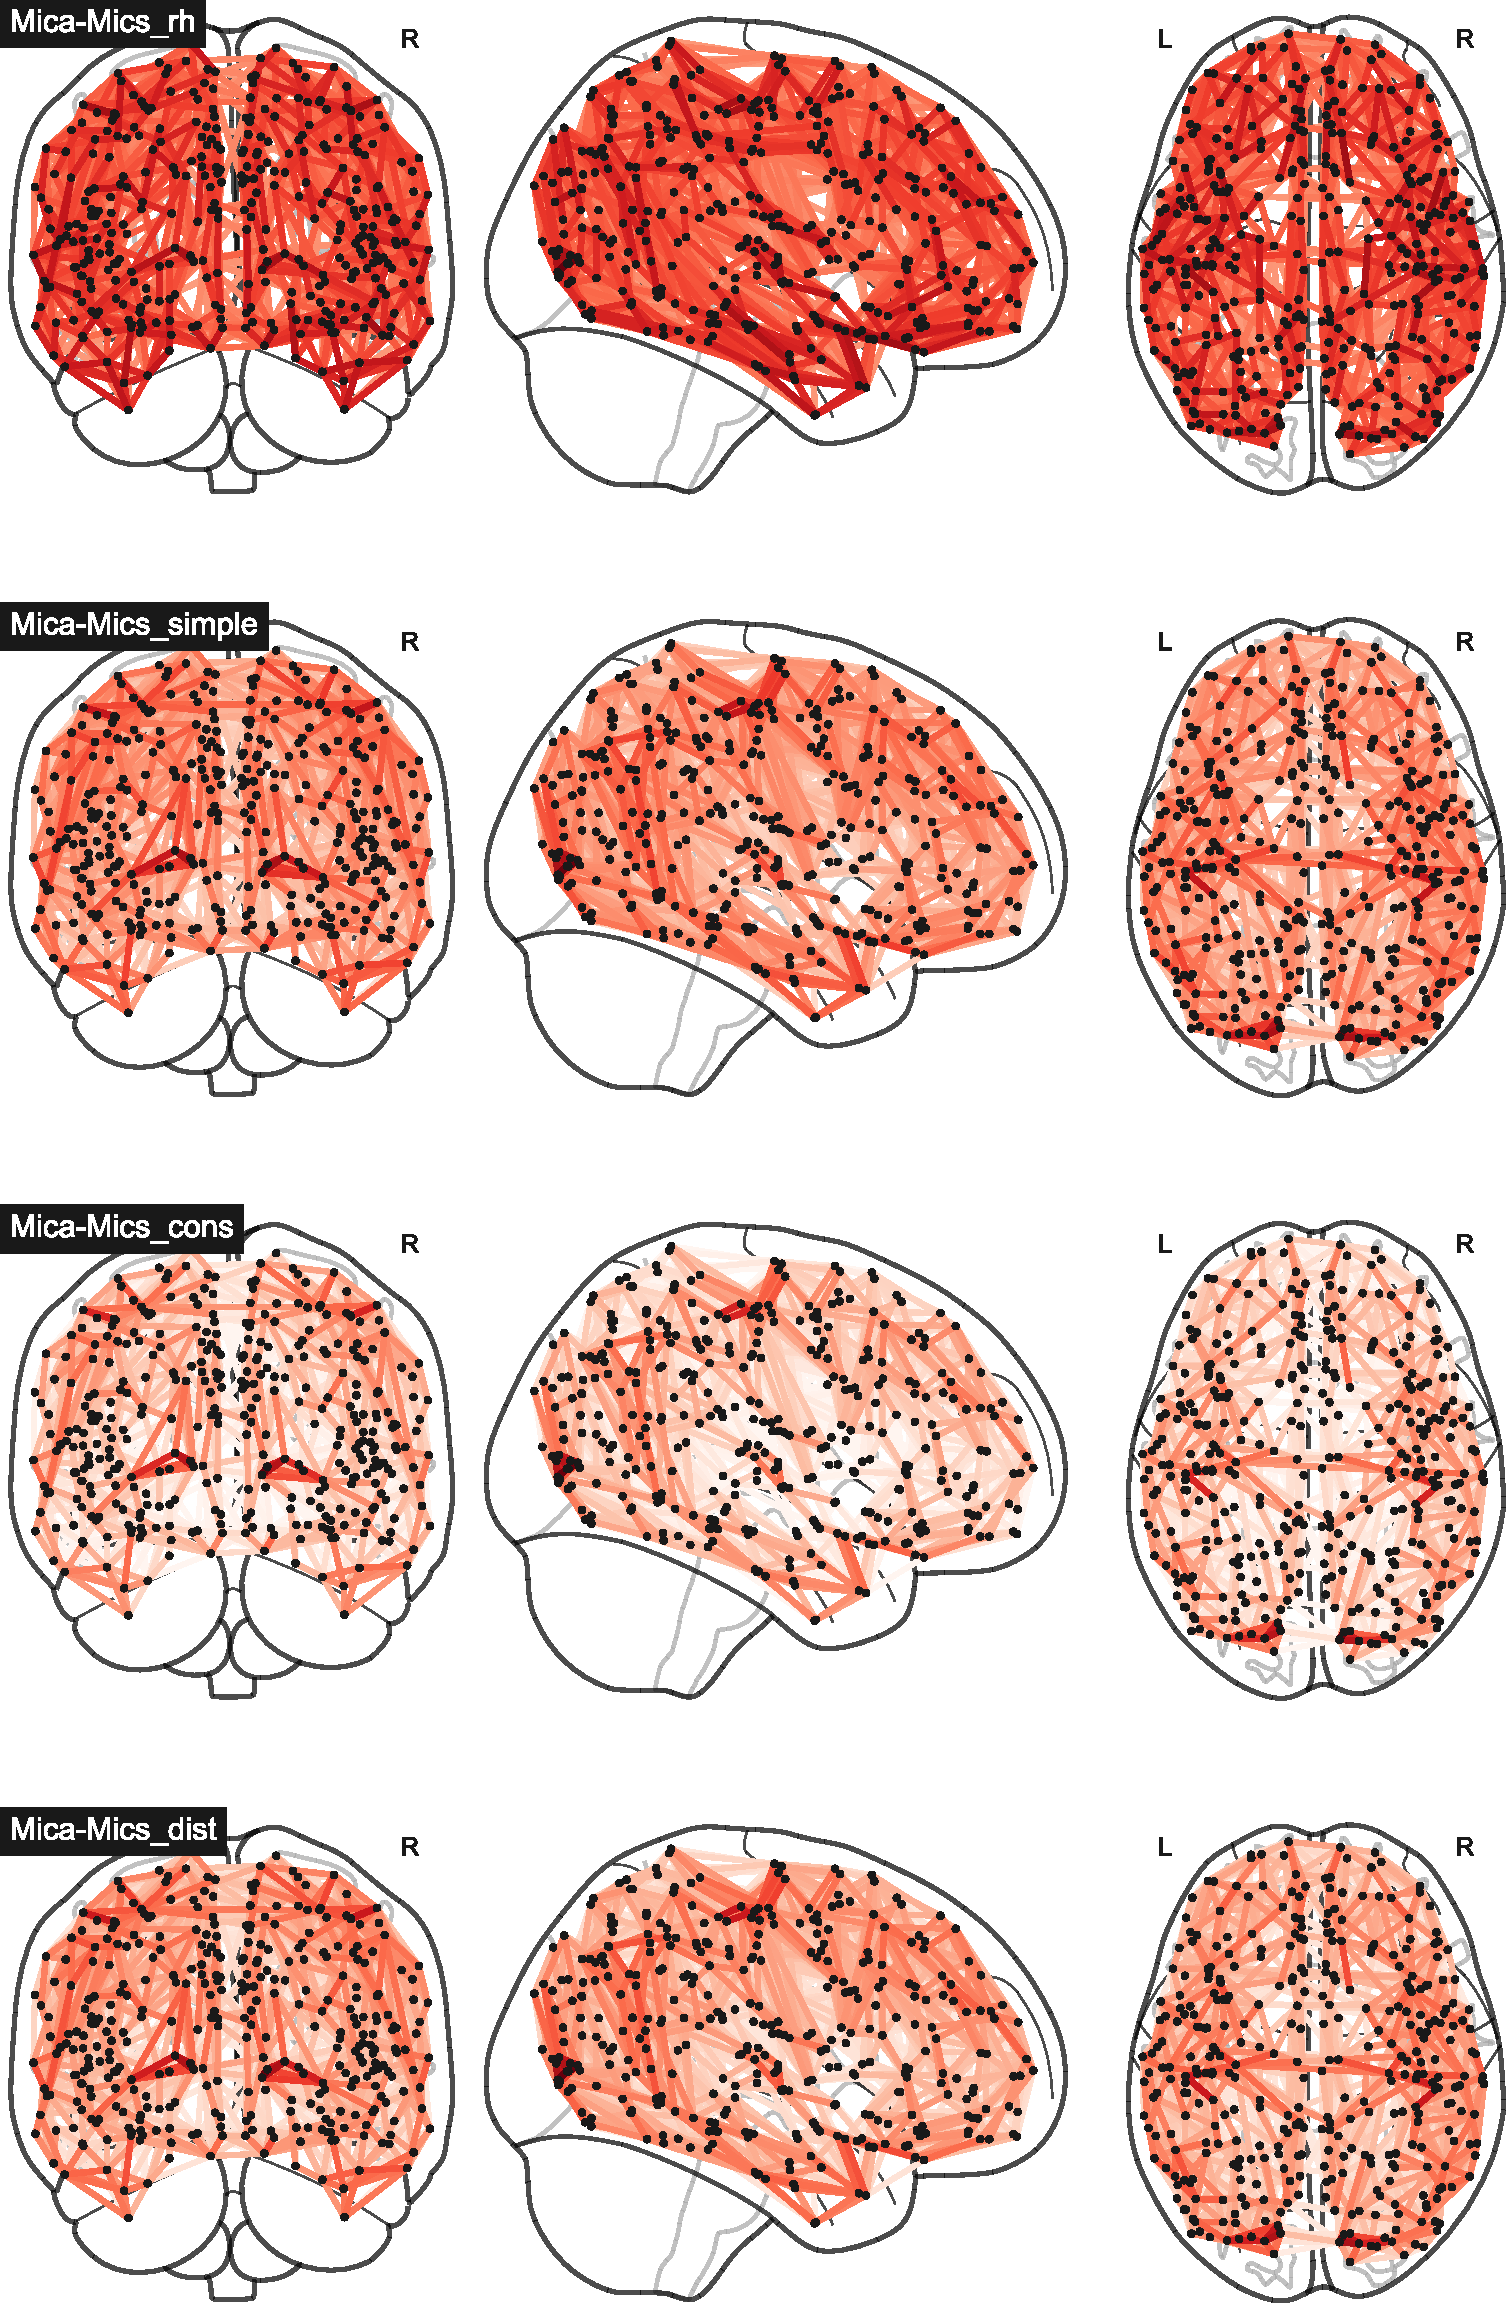
\includegraphics[width=0.9\textwidth]{images/compare_sc/connectomes_brain_thesis.pdf}
  \end{center}
  \caption[Connectome differences based on preprocessing method]{Connectome differences based on preprocessing method for Glasser parcellation, Mica-Mics dataset, edge weighted min-max normalized, plotted 3500 strongest edges.}
  \label{fig:edge_weights}
\end{figure}

\subsubsection{Edge lengths}

\TODO[Pro obyčejný consensu jsou tam spíš kratší hrany než pro ty jiné? Ale dist-dep se nijak výrazně neliší od ostatních, což je jiné, než píšou v tom článku.]

\section{Data sources}

\TODO[že podle toho, z jakého zdroje ta data jsou, vypadají různě]